% Copyright 2024 Jay Jay Billings. Some rights reserved.
\documentclass{article}
\usepackage{graphicx} % Required for inserting images
\usepackage{hyperref}
\usepackage{tabularx}
\usepackage{dirtytalk}

\title{Outliving your mind, part 3: No Rocking Chair}
\author{Jay Jay Billings, Ph.D.}
\date{\today}

%In this post, I'll talk about ways families can get help to support their loved ones, including public and private organizations, social support services, legal support for elder care, how and when to engage law enforcement, and how to have tough conversations with family members.

\begin{document}

\maketitle

\begin{center}
\textit{I don't need your rockin' chair, your Geritol or your medicare...}

\hspace*{\fill} - George Jones
\end{center}

\textit{In my \href{https://jayjaybillings.com/2023/07/06/outliving-your-mind-part-1-the-secret/}{last post} on my father's battle with dementia, I shared how his symptoms progressed over time. In this post, I'll talk about how families can get help.}

Key narrative points:
1. In an ideal world, there's tons of help for dementia.
2. We like to think everyone is prepared and going to be in that ideal world, but the truth is an enormous amount of people are fucked and never do anything about end-of-life health care or estate planning.
3. Dad never prepared for anything - he was in the second group.

ROCKING CHAIRS!!!!

\href{https://jayjaybillings.com/2016/08/18/family-rocking-chairs/s}{rocking chairs}

\section*{Public Organizations}

\section*{Private Facilities}

\section*{Legal Support}

\section*{When to Call the Po-Po}

\section*{Talking to Family}



\begin{figure}[h]
\caption{A very rare picture of my father in a rocking chair in 1993 or so. Also pictured: me (bottom left in the green shirt) and two of my brothers.}
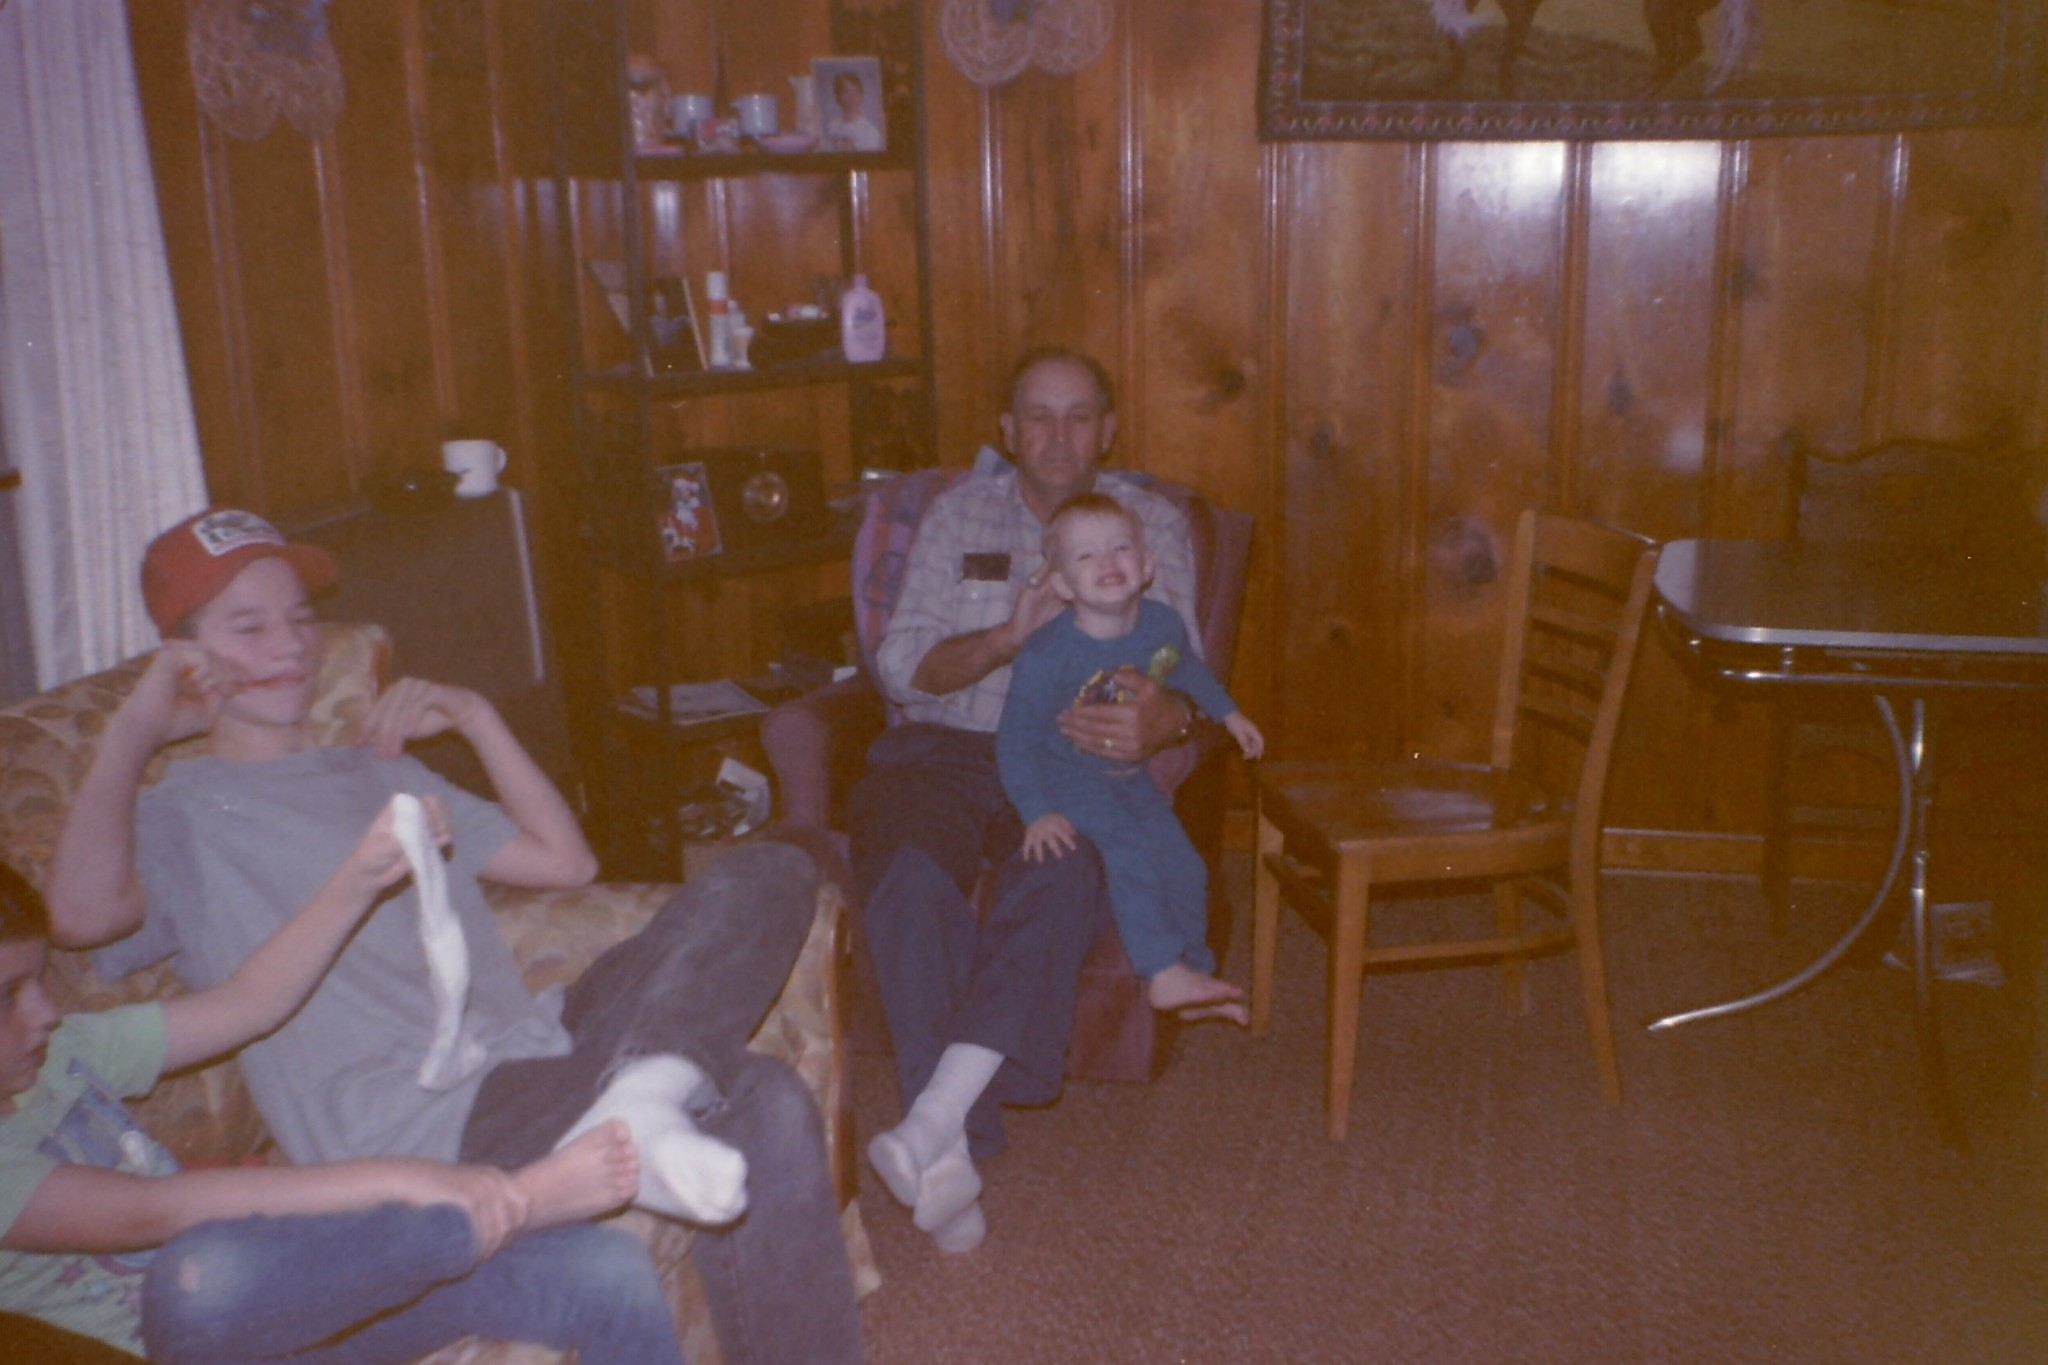
\includegraphics[width=\textwidth]{oym-p3-rocking-chairs/assets/PICT0043.JPG}
\label{rockingChair}
\end{figure}

\section*{Next Time}

Thanks for reading the third part of my series about my father’s struggles with cognitive decline and what we did to help him. I hope you’ll come back to read the next part, in which I'll discuss... 

I would especially like to thank my wonderful wife Paige for her support, Paige and my friend Brandon Nipper for their reviews of my draft, Michael Phelan for encouraging me to finish this article, and those who reached out after the earlier articles with kind words of encouragement and gratitude. 

\end{document}
